%\documentclass[11pt, twocolumn]{article}
\documentclass[final,leqno,onefignum,onetabnum]{siamart}

\usepackage{lingmacros}
\usepackage{tree-dvips}
\usepackage{graphicx}
\usepackage{amsmath}
\usepackage{amssymb}
\usepackage{tikz}
\usepackage{color}

\begin{document}

\title{Performance Evaluation of Automatic Differentiation Algorithms for Hessian Computation}
\maketitle

\section*{Introduction}
The second order derivative of a scalar function, i.e, the Hessian matrix, plays 
an important role in many applications. 
Several Automatic Differentiation (AD)-based Hessian evaluation algorithms have been proposed and implemented in the literature. While the high-level differences between the algorithms is generally understood, the detailed behavior of the algorithms and their performance characterization with respect to the structure and complexity of the computer code  representing the function to be differentiated has not been systematically studied and understood. In this work, we design a synthetic function that allows us to change the structural properties of the function by tuning parameters, and we use the designed function to study the performance of four different Hessian computation algorithms and the sensitivity of the performance to variations in those structural properties.

\section*{Algorithms}

We study three different approaches for Hessian evaluation. The first approach in turn has two variants, and so in total we consider four algorithms. In all four algorithms, 
the sparsity available in the final Hessian is exploited; that is, computing with and storing zero entries is avoided. All four of the algorithms compared are implemented with the operator overloading parameter. 

{\bf (i) Compression-based methods. }
The first two methods we study are based on the {\em forward-over-reverse mode}, or {\em Second-Order-Adjoint-Mode (SOAM)}, of Automatic Differentiation~\cite{griewank2008evaluating, naumann2012art}. Each run of a forward-over-reverse mode gives a Hessian-vector product $Hv$. Thus a trivial approach to get the entire Hessian matrix is to run the forward-over-reverse mode $n$ times, where $n$ is the number of columns in the Hessian and each run evaluates the $i$-th column of the Hessian, $He_i$. This approach is clearly not efficient  when the Hessian is sparse.  Therefore a compression-based method is used instead \cite{gebremedhin2009efficient}. 

The idea behind the compression-based approach is to determine an $n$ by $p$ seed matrix $S$
that encodes the set columns of the Hessian that can be ``compressed" together and evaluated via one Hessian-vector product. The seed matrix is typically obtained by
coloring the graph associated with the sparsity pattern of the Hessian. 
The number of columns $p$ in the seed matrix is exactly the number of colors needed. 
In this manner, only $p$ Hessian-vector products, instead of $n \gg p$ Hessan-vector products, is needed to obtain a compressed version of the Hessian. The desired Hessian is then obtained via a suitable recovery step.  

Depending on how the recovery step is performed, two different kinds of coloring are needed in the determination of the seed matrix. If the recovery is direct (no further arithmetic is involved in obtaining entries of the original Hessian),  {\em star} coloring is the needed coloring;
and if the recovery is indirect (entries of the original Hessian are obtained via substitutions), {\em acyclic} coloring is needed. In what follows, we refer to these two approaches  as {\tt Direct} and {\tt Indirect} respectively. We use the implementations in {\tt ADOL-C} \cite{walther2009getting} and {\tt ColPack} \cite{gebremedhin2013colpack}, in which {\tt ADOL-C} is responsible for the routines corresponding to computing the sparsity pattern and evaluating the compressed Hessian, and {\tt COlPack} is responsible for the routines  corresponding to coloring the adjacency graph and recovery the Hessian from the compressed representation.

{\bf (ii) Taylor coefficient based method. } 
The third Hessian evaluation method  we study  corresponds to evaluating the Hessian by propagating a family of second order Taylor coefficients~\cite{griewank2000evaluating}. 
By assigning pre-calculated initial values for each Taylor series, each entry in the Hessian matrix  can be determined by a linear combination of the final Taylor coefficients. Each initial value is called a {\em direction}.
The complexity of evaluating the Hessian using this method is proportional to a combination of $n^2$ and the complexity of the objective function. The complexity can be made proportional to $nnz$ and the complexity of the objective function, where $nnz$ is the number of non-zeros in the final Hessian matrix, by only evaluating those non-zero entries.
%The complexity of this method is $O(n^2)$. And if we know the sparsity pattern of the final Hessian matrix, the complexity can be reduced to $O(nnz)$ where $nnz$ is the number of non-zeros in the final Hessian matrix by only evaluating those non-zero entries.
We use the implementation in {\tt Rapsodia}~\cite{charpentier2009fast} and provide a patch which allows {\tt Rapsodia} to only evaluate the non-zero entries in the Hessian matrix with pre-determined sparsity pattern information. For the latter information, we use the sparsity pattern computed by {\tt ADOL-C}. The design philosophy of {\tt Rapsodia} is to use flat code to evaluate the Taylor coefficients for all directions. Given the number of directions, {\tt Rapsodia} explicitly generates this flat code. As we will show, when the number of directions is large, the generated code is very large and compilation takes huge amounts of time (several hours even for a moderate size problem), making the method infeasible. 

{\bf (iii) Live variable based method. }
The last method we study is second order reverse mode based on the {\em live variables} approach \cite{wang2016capitalizing}. The key idea in the algorithm is to extend a useful invariant in reverse mode AD into the second order. In particular, the insight is that, at each point, the intermediate state of the reverse mode algorithm is the derivative of an equivalent function with respect to the live variable set at that point. The equivalent function is defined by the single assignment codes processed in earlier steps. The complexity of this method is proportional to the size of live variable sets and the complexity of the objective function. We implement this algorithm in a tool we called {\tt ReverseAD} and uses this implementation in the comparison.

\section*{Design of test cases}

We construct testcases specially designed to enable in-depth empirical analysis of {\em structural factors} that determine the performance of the  different Hessian algorithms. 
To construct the testcases, we wrote a simple code that works as follows. 
Let the number of rows in the target Hessian matrix be $n$, and let the average number of nonzeros per row, $\bar{\rho}$, be fixed.
In a loop over the $n$ rows, we randomly pick $\frac{\bar{\rho}}{2}$ column indices $j$ and create a nonzero entry in the location $H(i,j)$. During the creation, we duplicate $s$ copies of $x[i]$ to ensure that the size of live variable sets during the function evaluation be $s$ for the most of the time. We also let $x[i]$ to pass through $k$ identity functions to make sure the test function covers a variety of kinds of operators and elementary functions. This also provides us with a way to control the complexity of the function evaluation. Each identity function is randomly chosen among six pre-determined forms. 

All random numbers are generated by a deterministic random number generator. Thus we can reproduce the function evaluations by giving the same initial seed.

With this setting, we can control the number of rows in the Hessian matrix $n$, the density/sparsity of the Hessian $\rho$, and the complexity of the function evaluation $k$, and the size of live variable sets during the function evaluation $s$.

%\appendix
%\section*
{\bf Details of The Synthetic Function. }
The synthetic function has the following mathematical form:
\begin{eqnarray*}
y &=& \sum\limits_{i=1}^{n} \sum\limits_{j=1}^{\rho/2} z_i * t_i \\ 
z_i &=& ID_k \circ \cdots \circ ID_1 (x_i), 1 \le i \le n, \\
t_i &=& \sum\limits_{j=1}^{\rho/2} x_{r_j} + \sum\limits_{j=1}^{s} x_{i_j}, x_{i_j} = x_i \\
\end{eqnarray*}
in which $ID_j$ is an identity function in one of the following $6$ forms:
\begin{eqnarray*}
ID(z) = 
\begin{cases}
\sqrt{z * z}, \\
2.0 + z - 2.0, \\
z * 2.0 * 0.5, \\
\log \exp(z), \\
1.0 / (1.0 / z), \\
sin(asin(z)). \\
\end{cases}
\end{eqnarray*}
$x_{i_j}$ are $s$ duplicated variables for $x_i$ to make the size of live variable set at least to be $s$. And by changing $k$, we can change the complexity of the function while keep the function value unchanged.




\section*{Results}

\paragraph{(a) General Runtime} We first use some small tests to get a general sense of the performance of the algorithms. We set $\rho = 6$, $k = 30$ and $s = 30$. 
Table~\ref{tab:general} lists the results we obtained when
we run the four algorithms with different values of $n$.  The observation here is that
{\tt Rapsodia} takes much longer time compared with the other three methods, and it also takes hours to compile the ``flat-code'' when there are more than $10,000$ directions. 
So we excludes this method from further tests we report on.
\begin{table}[htbp]
\begin{center}
\begin{tabular}{ | c | r | r | r | r | r |}
\hline
$n$ & $\#nnz$ in $H$ & {\tt Direct} & {\tt Indirect} & {\tt Rapsodia} & {\tt ReverseAD} \\
\hline
$2,000$ & 7,990 & 2.332 & 1.996 & 11.703 & 0.795 \\
$3,000$ & 11,989 & 3.671 & 3.258 & 26.808 & 1.207\\
\hline 
\end{tabular}
\end{center}
\caption{General Runtime for {\tt Direct}, {\tt Indirect}, {\tt Rapsodia} and {\tt ReverseAD}.}
\label{tab:general}
\end{table}

\paragraph{(b) Function Complexity} 
Our goal here is to see how the performance changes as the function complexity is varied.
We set $n = 20,000$, $\rho = 6$, $s = 30$, and vary $k$ from $20$ to $60$. 
The results we obtained are summarized in Table~\ref{tab:complexity}.
We found that the runtime of {\tt Direct} and {\tt Indirect} increases super-linearly with increase in the function complexity. Further, we found that that more than $90\%$ (or $99\%$ in the last two tests) of the time is spent in the sparsity pattern detection procedure, see Figure~\ref{fig:complexity-percentile}. It is likely that our synthetic function is among the ``worst-case" instances for the current sparsity pattern detection procedure implemented in ADOL-C.  Finally, we see that the runtime of {\tt ReverseAD} is within the same order of the function complexity.
\begin{table*}[htbp]
\begin{center}
\begin{tabular}{ | c | r | r | r | r | r |}
\hline
 & $k=$ 20 & 30 & 40 & 50 & 60 \\
\hline
{\tt Direct} & 9.325 & 25.268 &181.435 &1765.766 & 14114.265\\
{\tt Indirect} & 7.138 & 22.007 & 177.539 & 1760.754 & 14124.760\\
{\tt ReverseAD}  & 6.367 & 8.220 & 9.824 & 11.763 & 13.242\\
\hline 
\end{tabular}
\caption{Runtime for {\tt Direct}, {\tt Indirect} and {\tt ReverseAD} with different function complexity.}
\label{tab:complexity}
\end{center}
\end{table*}

\begin{figure}[htbp]
        \centering
        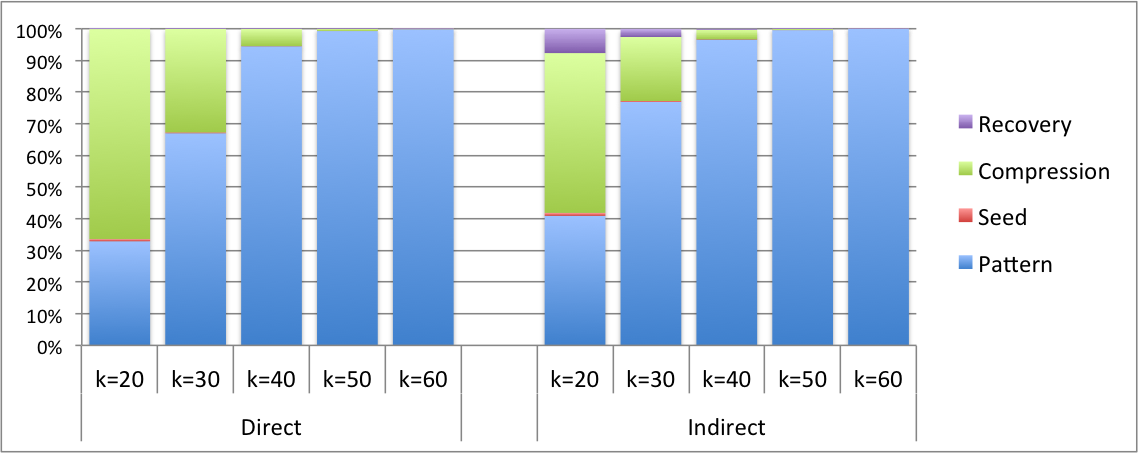
\includegraphics[width=0.85\textwidth]{figures/pb}
        \caption{Percentile breakdown for {\tt Direct} and {\tt Indirect} with different function complexity.}
        \label{fig:complexity-percentile}
\end{figure}

\paragraph{(c) Size of Live Variables} 
Here we want to see how the performance changes as we vary the size of the live variable set.
We fix $n = 20,000$, $\rho = 6$, $k = 30$ and changes $s$ from $20$ to $60$. The results (summarized in Table~\ref{tab:live} suggest that performance of {\tt ReverseAD} is much more sensitive to the size of live variable set than the other two algorithms. This is in accordance with our expectation and the complexity analysis of the algorithm.
\begin{table*}[htbp]
\begin{center}
\begin{tabular}{ | c | r | r | r | r | r |}
\hline
& $s=$ 20 & 30 & 40 & 50 & 60 \\
\hline
{\tt Direct} & 23.653 & 25.138 & 26.484 & 27.666 & 29.208\\
{\tt Indirect} & 21.071 & 22.310 & 23.110 & 23.843 & 25.075\\
{\tt ReverseAD} & 6.137 & 8.087 & 10.207 & 12.507 & 14.421\\
\hline 
\end{tabular}
\caption{Runtime for {\tt Direct}, {\tt Indirect} and {\tt ReverseAD} with different size of live variables.}
\label{tab:live}
\end{center}
\end{table*}

\paragraph{(d) Sparsity/Density} 
Here we fix $s$ to be  $30$, and perform tests on three sets of settings: $n=15,000$, $\rho = 8$, $k=40$; $n=20,000$, $\rho=6$, $k=30$; and $n=30,000$, $\rho=4$, $k=20$. 
We choose those parameters so that the complexity of the function evaluation and the total number of non-zeros in the final Hessian matrix are roughly the same across the different settings. 
Table~\ref{tab:sparsity} lists the results we obtained.
We see that the runtime of {\tt Direct} and {\tt Indirect} increases as the density of the Hessian matrix increases. 
Again, this is due to the sparsity pattern detection procedure, which takes lesser time as the density decreases, as the breakdown in Figure~\ref{fig:sparsity-percentile} shows.
Finally, we see that {\tt ReverseAD} takes more time when the density of the Hessian matrix increases, but the growth rate is relatively small.
\begin{table*}[htbp]
\begin{center}
\begin{tabular}{ | c | r | r | r |}
\hline
& $n=$ $15,000$ & $20,000$ & $30,000$\\
\hline
{\tt Direct} & 139.841 & 25.745 & 12.833\\
{\tt Indirect} & 134.210 & 22.232 & 9.664 \\
{\tt ReverseAD} & 7.616 & 8.634 & 9.745\\
\hline 
\end{tabular}
\caption{Runtime for {\tt Direct}, {\tt Indirect} and {\tt ReverseAD} with different sparsity/density.}
\label{tab:sparsity}
\end{center}
\end{table*}

\begin{figure}[htbp]
        \centering
        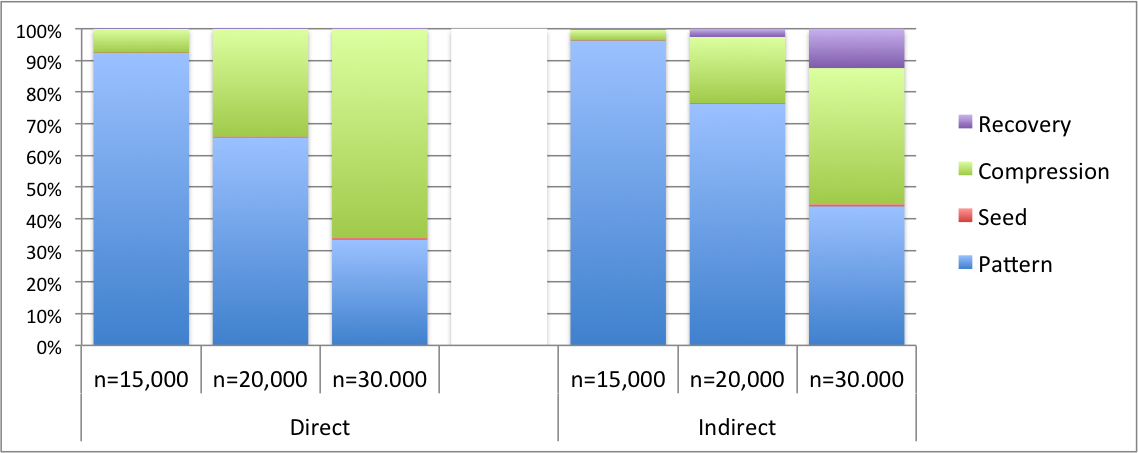
\includegraphics[width=0.65\textwidth]{figures/pd}
        \caption{Percentile breakdown for {\tt Direct} and {\tt Indirect} with different sparsity/density.}
        \label{fig:sparsity-percentile}
\end{figure}

\section*{Conclusion}
By comparing the performance of the four different Hessian evaluating algorithms, we found that the approach in {\tt Rapsodia} is feasible only when evaluating derivatives for function with a few number of independent variables. We also found that the bottleneck in the compression based methods is mainly the sparsity pattern step. The {\tt ReverseAD} approach is more stable and efficient approach in most cases. 


\bibliographystyle{abbrv}
\bibliography{adbib}



\end{document}